%% Uji dasar Fase 2: halaman, font, spasi, judul bab, tabel/gambar, penomoran Bab.n.
%% Kompilasi: pdflatex -interaction=nonstopmode uji-dasar.tex  (2x)
\documentclass[jenis=skripsi,mode=laporan,jenjang=sarjana,sitasi=apa,logo=logo-placeholder]{unnes-ta}

\identitas{
  judul      = {PENGUJIAN DASAR KELAS unnes-ta UNTUK TUGAS AKHIR},
  nama       = {Nama Mahasiswa},
  nim        = {1234567890},
  prodi      = {Pendidikan Teknik Informatika},
  fakultas   = {Fakultas Teknik},
  gelar      = {Sarjana Pendidikan},
  tahun      = {2026},
  pembimbinga      = {Dr. Pembimbing Satu, M.Kom.},
  pembimbinganip   = {198001012005011001},
}

\begin{document}
\bagianawal
\chapter*{HALAMAN UJI DASAR}
Dokumen ini hanya untuk menguji mekanisme kelas: margin, tipe huruf, spasi, penomoran
halaman, bentuk judul bab, caption tabel/gambar, dan penomoran bertingkat Bab.n.

\tableofcontents

\bagianutama
\chapter{PENDAHULUAN}
\section{Latar Belakang}
Panduan tugas akhir Universitas Negeri Semarang menetapkan tipe huruf Times New Roman
ukuran 12 pt, jarak baris 1,5 spasi untuk laporan dan 1,15 spasi untuk proposal,
ukuran kertas A4 satu kolom, perataan teks rata kiri-kanan, serta tata letak halaman
dengan margin kiri 4 cm, kanan 3 cm, atas 3 cm, dan bawah 3 cm. Pengujian ini memastikan
kelas unnes-ta mematuhi seluruh ketentuan tersebut sekaligus menguji perilaku perataan
teks pada paragraf panjang berbahasa Indonesia agar terlihat apakah terjadi pemenggalan
kata yang berlebihan atau jarak antarkata yang terlalu renggang.

\subsection{Subbagian Uji}
Subbagian ini menguji bentuk dan penomoran subbab, termasuk subbagian bertingkat lanjut
yang seharusnya tetap terdaftar sampai tingkat kedua pada daftar isi.

\subsubsection{Sub-subbagian Uji}
Tingkat ketiga tetap bernomor tetapi tidak lagi tercantum di daftar isi.

\chapter{METODE PENELITIAN}
\section{Tabel dan Gambar}
Tabel dan gambar diuji untuk memastikan label berbahasa Indonesia dan penomoran mengikuti
nomor bab.

\begin{table}[htbp]
  \centering
  \caption{Hasil pengujian margin halaman}
  \label{tab:margin}
  \begin{tabular}{lcc}
    \toprule
    Aturan panduan & Nilai wajib & Hasil uji \\
    \midrule
    Margin kiri   & 4 cm & 4 cm \\
    Margin kanan  & 3 cm & 3 cm \\
    Margin atas   & 3 cm & 3 cm \\
    Margin bawah  & 3 cm & 3 cm \\
    \bottomrule
  \end{tabular}
  \sumber{Panduan TA UNNES 2024 hal. 16; pengukuran hasil kompilasi}
\end{table}

\begin{figure}[htbp]
  \centering
  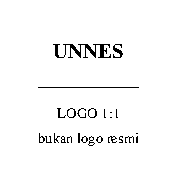
\includegraphics[width=3cm]{../logo/logo-placeholder}
  \caption{Contoh penempatan gambar dengan judul di bawah gambar}
  \label{gam:uji}
  \sumber{Dokumentasi penulis}
\end{figure}

\section{Persamaan}
Penomoran persamaan juga mengikuti nomor bab:
\begin{equation}
  \label{eq:uji}
  y = \beta_0 + \beta_1 x + \varepsilon
\end{equation}

\section{Tabel Panjang}
\begin{tabelpanjang}{cl}{Contoh tabel panjang lintas halaman}{tab:panjang}
  \toprule
  Kode & Keterangan \\
  \midrule
  \endhead
  A01 & Baris uji pertama \\
  A02 & Baris uji kedua \\
  A03 & Baris uji ketiga \\
\end{tabelpanjang}

\begin{thebibliography}{9}
\bibitem[Geraldi \& S{\"o}derlund(2017)]{geraldi2017project}
  Geraldi, J., \& S{\"o}derlund, J. (2017). Project studies: What it is and where it's going.
  \textit{International Journal of Project Management}, 6(1).
\end{thebibliography}
\end{document}
